\documentclass[aspectratio=1610]{beamer}
\title[Hall's Ray]{Hall's Ray\\of the Markov and Lagrange Spectra}
\author{Oleg Smirnov}
\institute{Higher School of Economics}
\date{2022}

\newcommand{\N}{\mathbb{N}}
\newcommand{\Z}{\mathbb{Z}}
\newcommand{\R}{\mathbb{R}}
\newcommand{\Q}{\mathbb{Q}}
\newcommand{\M}{\mathcal{M}}
\renewcommand{\l}{\lambda}
\newcommand{\m}{\mu}
\newcommand{\g}{\upgamma}
\renewcommand{\d}{\delta}
\newcommand{\D}{\Delta}


\usepackage{amsfonts, amsmath, amssymb, amsthm, array, hhline, amscd, mathtools}
\usepackage{xcolor}

\graphicspath{{media/}}
\DeclareGraphicsExtensions{.pdf,.png,.jpg}

\begin{document}

\frame{\titlepage}

\begin{frame}
\frametitle{Diophantine approximations}

Consider $\alpha \in \R \backslash \Q$.

We want to approximate $\alpha$ with rational $\frac{p}{q}$, minimizing the distance
\begin{equation*}
	\left|
		\alpha - \dfrac{p}{q}
	\right|.
\end{equation*}

Some approximations are better than other:
\begin{equation*}
	\begin{aligned}
		\left|
			\pi - \dfrac{314}{100}
		\right| & \approx 1.5 \cdot 10^{-3},\\
		\left|
			\pi - \dfrac{355}{113}
		\right| & \approx 2.6 \cdot 10^{-7}.		
	\end{aligned}
\end{equation*}

How do we find good diophantine approximations?

\end{frame}

\begin{frame}
\frametitle{Continued fractions}

Representing $\alpha$ as a continued fraction:
\begin{equation*}
	\alpha =
	[a_0; a_1, a_2, ...] =
	a_0 + \dfrac{1}{\normalsize a_1 + \dfrac{1}{a_2 + \dfrac{1}{\ddots}}},\;\;
	a_0 \in \mathbb{Z},\; a_1, a_2, ... \in \mathbb{N}.
\end{equation*}

The continued fraction produces infinitely many rational convergents of $\alpha$:
\begin{equation*}
	\alpha_n = \dfrac{P_n}{Q_n} = [a_0; a_1, a_2, ..., a_n].
\end{equation*}

The sequence $\{\alpha_n\}$ converges to $\alpha$:
\begin{figure}[c]
	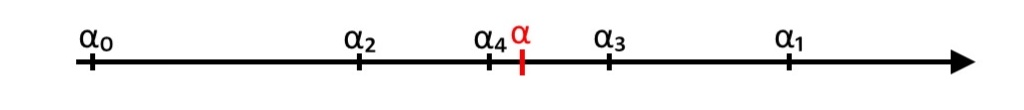
\includegraphics[width=0.8\textwidth]{convergents}
\end{figure}

\end{frame}

\begin{frame}
\frametitle{Convergents}

The convergents of a continued fraction give the best diophantine approximations.

For example:

\begin{equation*}
	\begin{aligned}
			\pi & =
			3 + \cfrac{1}{7 + \cfrac{1}{15 + \cfrac{1}{1 \color{red} + \cfrac{1}{292 + \cfrac{1}{1 + \cfrac{1}{\ddots}}}}}},\\
			\dfrac{355}{113} & =
			3 + \cfrac{1}{7 + \cfrac{1}{15 + \cfrac{1}{1}}}.
	\end{aligned}
\end{equation*}

\end{frame}

\begin{frame}
\frametitle{Hurwitz theorem}

The following theorem describes the best possible quality of approximation for an arbitrary $\alpha$:

\begin{theorem}[Hurwitz]
	\label{theorem_hurwitz}
	For any irrational $\alpha$,
	there exist infinitely many rationals $\frac{p}{q}$ such that
	\begin{equation*}
		\label{condition_hurwitz}
		\left| \alpha - \frac{p}{q} \right| < \dfrac{1}{\sqrt{5} q^2}.
	\end{equation*}
	On the other hand, for any $c > \sqrt{5}$ the inequality
	\begin{equation}\label{eq:markov-inequality}
		\left| \varphi - \frac{p}{q} \right| < \dfrac{1}{c q^2}.
	\end{equation}
	has only finitely many solutions,
	where $\varphi = \frac{1 + \sqrt{5}}{2}$
	is the golden ratio.
\end{theorem}

\end{frame}

\begin{frame}
\frametitle{Markov value}

\begin{definition}
	Let the Markov value $M(\alpha)$ of an irrational $\alpha$ be
	the smallest constant $c$ such that inequality (\ref{eq:markov-inequality}) has infinitely many solutions.
\end{definition}

%By Hurwitz theorem, $M(\alpha) \geqslant \sqrt{5}$ for all $\alpha$ and $M(\varphi) = \sqrt{5}$.

Markov values allow us to introduce Lagrange spectrum.

\begin{definition}
	Lagrange spectrum $L$ is the set of the Markov values over all irrationals:
	\begin{equation*}
		L \coloneqq \{M(\alpha) \mid \alpha \in \R \backslash \Q\}.
	\end{equation*}
\end{definition}

\end{frame}

\begin{frame}
\frametitle{Lagrange spectrum}

\begin{definition}
	$\mathcal{M}$ stands for a double-infinite sequence of positive integers:
	\begin{equation*}
		\mathcal{M} =
		\left(..., a_{-2}, a_{-1}, a_0, a_1, a_2, ...\right)
		\in \mathbb{N}^\mathbb{Z}.
	\end{equation*}
\end{definition}

\begin{definition}
	The height function is defined as
	\begin{equation*}
		\begin{gathered}
			f : \mathbb{N}^\mathbb{Z} \rightarrow \mathbb{R},\\
			f(\mathcal{M}) = a_0 + [0; a_{-1}, a_{-2}, ...] + [0; a_{1}, a_{2}, ...].
		\end{gathered}
	\end{equation*}
\end{definition}

\begin{definition}
	The shift function is defined as
	\begin{equation*}
		\begin{gathered}
			\sigma : \mathbb{N}^\mathbb{Z} \rightarrow \mathbb{N}^\mathbb{Z},\\
			\sigma(... a_{-2} a_{-1} \underline{a_0} a_1 a_2 ...) = ... a_{-1} a_{0} \underline{a_1} a_2 a_3 ...
		\end{gathered}
	\end{equation*}
\end{definition}

\end{frame}

\begin{frame}
\frametitle{Lagrange spectrum}

We are now ready to give an alternative definition for the Lagrange spectrum.

\begin{definition}
	Let the Lagrange value of a double-infinite sequence $\mathcal{M}$ be
	\begin{equation*}
		\ell(\mathcal{M})
		\coloneqq \limsup\limits_{k \rightarrow + \infty} f(\sigma^k \mathcal{M}).
	\end{equation*}
\end{definition}

\begin{definition}
	Lagrange spectrum is the set of Lagrange values over all double-infinite sequences:
	\begin{equation*}
		L \coloneqq \{ \ell(\mathcal{M}) \mid
		\mathcal{M} \in \mathbb{N}^\mathbb{Z} \}.
	\end{equation*}
\end{definition}

\end{frame}

\begin{frame}
\frametitle{Lagrange spectrum geometry}

\end{frame}


\end{document}